\documentclass[12pt,a4paper]{article}
\usepackage{hyperref}
\usepackage{csquotes}
\usepackage{float}
\usepackage{graphicx}
\usepackage{easyReview}
\usepackage{wrapfig}
\usepackage{amsmath,mathtools, nccmath}
\usepackage{siunitx}

\newcommand{\imagesource}[1]{{\footnotesize Source: #1}}
\renewcommand{\familydefault}{\sfdefault}

\graphicspath{ {images/} }

\hypersetup{
	colorlinks=true,
	linkcolor=blue,
	filecolor=magenta,      
	urlcolor=cyan,
	pdftitle={What are important features to have in a dataset?},
	pdfpagemode=FullScreen,
}

\usepackage[
backend=biber,
style=apa,
]{biblatex}
\addbibresource{sources.bib}

\title{Brains 4 Building Human Satisfaction}
\author{Leander Oudakker, Maarten Donkersloot, Max Bogaers}
\date{\today}

\begin{document}
	
\maketitle

\pagebreak

\tableofcontents

\pagebreak

\listoffigures

\pagebreak

\section{Introduction}
The Dutch government aims for a 49\% reduction in greenhouse gas emissions in 2030 (compared to 1990). During the current government term, each year 30,000-50,000 existing homes need to be converted to make them gas-free, and the market should be ready to make 200,000 houses per year sustainable beyond 2021. The large-scale energy transition of the urban energy system faces multiple challenges, which calls for the active involvement of house owners and stakeholders across many sectors. 

To help in this endeavor the brains for buildings program was started. Focused on developing methods to harness big data from smart meters, building management systems and the Internet of Things devices, to reduce energy consumption, increase comfort, respond flexibly to user behavior and save on installation maintenance costs.

Within brains for buildings this could be done using machine learning and artificial intelligence, one project within brains for buildings is human-satisfaction. This branch is focused on finding out if AI can be used to get more information on the human-satisfaction within buildings and how we can use that information to better distribute our energy. For example only occupied areas off a building would be optimized for comfort.

We were tasked with making a start to this, we started the project with the following questions from our stakeholders:

\begin{itemize}
	\item What kind of data should we collect to be able to measure the comfort and wellbeing of the people? 
	
	\item How could we collect this data actively and passively to measure the comfort and wellbeing of the people? 
	
	\item What are the objective criteria we should match against? 
	
	\item Can we use machine learning to find patterns between the objective measurements and subjective comfort/wellbeing of the people? 
\end{itemize}

After much back and forth about scope and the aforementioned stakeholder questions we decided that our research paper will be focused on finding out what the best way is to involve machine learning in bettering the human satisfaction corresponding to the climate of a building. 
We will be finding this out through the following sub-questions:

\begin{itemize}
	\item What is human satisfaction?
	\item What are the alternatives to using machine learning to predict human satisfaction corresponding to the climate of a building?
	\item What are important features to have in a dataset?
\end{itemize}

\pagebreak

\section{What is human satisfaction?}
In this paper, there is a focus on trying to predict human satisfaction and gain insight into if someone would be satisfied currently or in the future and what could be done to improve said satisfaction.

Satisfaction and comfort go hand in hand, if someone's comfortable there's a high chance that he or she will also be satisfied by said space. However, comfort does limit our definition of satisfaction, it does not only relate to the ambient qualities of a room, like temperature, noise and light, but also to more abstract factors that we might not consider when just thinking about comfort.
(\cite{Comfort_in_architecture}) (\cite{Human_Wants})

Thus, a good description of how human satisfaction is defined within the paper is as follows.
\begin{displayquote}
	"A person's feelings of fulfillment or disappointment resulting from comparing perceived comfort with their own expectations and the ambient qualities of a room."
\end{displayquote}

\section{What are the alternatives to using machine learning to predict human satisfaction corresponding to the climate of a building?}
Before starting a project one should always look at the feasibility of the solution offered.This section explains what techniques can be used to predict human satisfaction and the corresponding advantages and disadvantages.

\subsection{Using mathematics to predict human satisfaction}
The prediction of thermal comfort using mathematics mostly expresses itself in formulas that predict or classify the thermal sensation of people in buildings. There are three main standards used for this:

\begin{itemize}
	\item The international standard ISO 7730 Ergonomics of the thermal environment - Analytical determination and interpretation of thermal comfort using calculation of the PMV and PPD indices and local thermal comfort criteria
	\item The European NEN-EN 15251 Indoor environmental input parameters for design and assessment of energy performance of buildings addressing indoor air quality, thermal environment, lighting and acoustics
	\item The American ASHRAE/ANSI Standard 55 – Thermal Environmental Conditions for Human Occupancy
\end{itemize}

These formulas take into account environmental variables such as: temperature, thermal radiation, humidity and airspeed, but also personal factors such as: level of activity and clothing insulation to predict if people are satisfied with the climate.

\subsubsection{Fanger method}
Predicted mean vote (PMV) and predicted percentage of dissatisfied (PPD) are indices used by the above-mentioned standards to measure thermal comfort. These indices come from the research done by the Danish professor Povl Ole Fanger on thermal comfort in the 1960's, and are based on the perception of a large group of people to factors such as metabolic rate, clothing insulation and environmental conditions (\cite{Fanger1972ThermalCA}).
\subsubsection{Predicted Mean Vote}
Predicted Mean Vote is an index that aims to predict the mean value of votes of a group of occupants on a seven-point thermal sensation scale ranging from -3 (cold) to +3 (hot). Where 0 is described as the thermal equilibrium, when an occupant’s internal heat production is the same as its heat loss.(\cite{fanger1970}) The formula to calculate PMV is : 
\[PMV = (0,303e^{-2.100*M}+0,028)\cdot[(M-W)-H-E_{c}-C_{res}-E_{res}]\]
where the different terms represent:
\begin{description}
	\item[M] the metabolic rate, in Watt per square meter (W/m2)
	\item[W] the effective mechanical power, in Watt per square meter (W/m2)
	\item[H] the sensitive heat losses
	\item[$E_{c}$] the heat exchange by evaporation on the skin
	\item[$C_{res}$] heat exchange by convection in breathing
	\item[$E_{res}$] the evaporative heat exchange in breathing
\end{description}
(\cite{Silva})

\begin{figure}[h]
	\caption{PPD Drawn Over PMV}
	\centering
	\begin{tabular}{ @{} r @{} }
		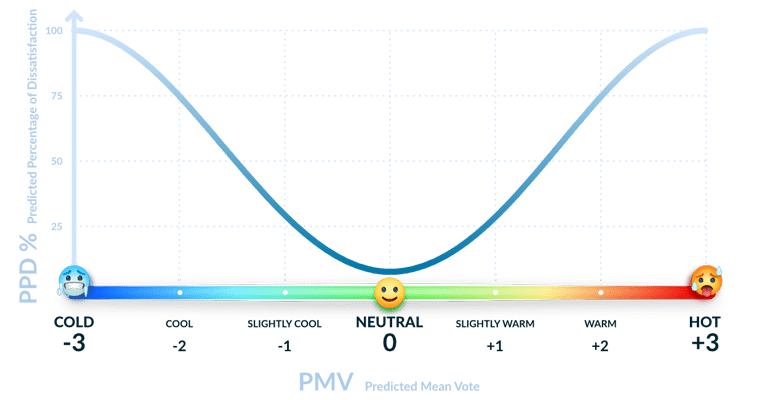
\includegraphics[width=0.75\textwidth]{pmv_ppd} \\
		\imagesource{\cite{guenther_2021}}
	\end{tabular}
\end{figure}

\subsubsection{Predicted Percentage of Dissatisfied}
Building on PMV there is PPD, PPD is an equation used to determine what percentage of people are satisfied with the room's climate. PPD essentially calculates the percentage of people predicted to experience local discomfort within a given space.
The PPD formula is as follows:
\[PPD = 100-95\cdot^{-(0.03353 \cdot PMV^{4} + 0.2179 \cdot PMV^{2})}\]
(\cite{fanger1970})
  
\subsubsection{Adaptive thermal comfort equations}
The equations that have been discussed up to this point have been static equations. These equations don't take into account variable's like temperature or humidity, like the following standards will.
\subsubsection{Standards}
Rather than just use the PMV and PPD calculations, most organizations use standards that integrate these calculations along with other factors to determine  the climate satisfaction in a room. The two most used standard of these are ASHRAE 55 and ISO 7730.


\subsubsection{ASHRAE standard 55}
"ANSI/ASHRAE Standard 55: Thermal Environmental Conditions for Human Occupancy" is the oldest of the three discussed standards, it was first published in 1966 by the American Society of Heating, Refrigerating and Air-Conditioning.	And was first expanded upon by P. O. Fanger  based on experiments done in the 1960s at the Kansas State University. This first standard was build on a basis of temperature and humidity, but through the years the standard grew to include things like PMV, PPD , Metabolic rate, air turbulence, clothing isolation, etc. (\cite{999821325502121}) Through the inclusion of these metrics ASHRAE 55 became the go-to standard for predicting the climate satisfaction in America. 
(\cite{ASHRAE})

\subsubsection{ISO 7730}
"ISO 7730: Ergonomics of the thermal environment - Analytical determination and interpretation of thermal comfort using calculation of the PMV and PPD indices and local thermal comfort criteria" is an international standard published by ISO, the ISO is an international standard setting organization founded in 1947. ISO works with 165 countries to set technical, industrial and commercial standards (\cite{iso_2021}). The 7730 standard presents methods for predicting the general thermal sensation and degree of thermal dissatisfaction of healthy people exposed to moderate thermal environments. This standard uses the same environmental  metrics as described by ASHRAE 55 but expands on them by also including cultural, national and geological factors. 
(\cite{ISO7730})


\subsection{Using ML to predict human satisfaction}
The alternative to using these mathematical formulas to predict human satisfaction is training a machine learning model to predict thermal comfort, but due to this being a new field of research there aren't many studies researching this topic. One of the few studies researching this is \add{(}\cite{LUO2020109776}\add{)}, this study used an ASHRAE database to train various machine learning models. But they were unable to achieve high accuracy using this method with the best algorithm only guessing it right about 66\% of the time. A problem  with this paper is that they used a static method of predicting thermal comfort which severely limits the data that can be used by the model. But studies using an adaptive model are uncommon there is one (\cite{CHAI2020109937}) but this study doesn't explain much about the parameters and hyperparameters of the machine learning models used. But they did find out their models where more accurate at predicting thermal comfort than using the PMV calculation.
 
\section{What are important features to have in a dataset?}
In order to make any kind of prediction we need to assess what features are necessary to predict our target, in this case that is the aforementioned human satisfaction. This section explains which features were considered and why, what features we ended up with and how we got those features.
\subsection{Feature research}
Before there can be any sort of benchmarking or modeling done there would need to be decided which features are of importance, why these features are of importance, if this data can be retrieved at Avans and what the alternatives are to not having data from Avans.

\subsubsection{The 9 foundations of a healthy building}
The Harvard school of public health wrote a report titled "The 9 foundations of a healthy building". The purpose of this report was to create actionable points which would improve a building's health. Even though the paper report's focus isn't on satisfaction it's a good resource for the kinds of data that are important to include the research.

This document notes the following foundational aspects:
\begin{itemize}
	\item Ventilation
	\item Air quality
	\item Water quality
	\item Thermal health
	\item Dust and pests
	\item Lighting and views
	\item Noise
	\item Moisture
	\item Safety and security
\end{itemize}
(\cite{9foundations})

Each of these features relates to climate/human satisfaction in their own ways, the next sections will describe how they affect the parameters.
(\cite{9foundations})

\subsubsection{Ventilation/Air quality}
Ventilation has a direct impact on air quality, less ventilation reduces that quality which can cause all kinds of issues. Some of the side effects could be irritation to the eyes, skin, nose and throat. This would obviously have a bad effect (and thus a good impact) on human satisfaction. 
(\cite{9foundations})

\subsubsection{Temperature}
Temperature has a significant impact on performance and health. In a previously done survey across Europe, the foremost complaint reported was a lack of thermal comfort. Furthermore, there have been studies conducted on how it impacts learning in students (specifically sixth grade), which concluded that students who have never experienced high indoor temperatures achieved more correct answers on tests. Additionally, high temperatures have been linked too negative moods, heart rate, respiratory symptoms and feelings of fatigue.

Furthermore, temperature has a direct correlation with humidity (humidity increases the temperature people feel), if the humidity is too high it would, for example, reduce the capacity for the body to cool itself, thus making us uncomfortable.
(\cite{9foundations})

\subsubsection{Water quality}
Water quality has a direct impact on health, if this quality is bad then small pieces of lead bioaccumulate in the body and affect our cognitive ability. Getting some kind of water quality reading would be a good secondary feature, it affects the satisfaction indirectly.
(\cite{9foundations})

\subsubsection{Lighting}
Light has a direct impact on health, specifically on your sleep schedule and metabolism. Lighting could be included in the study, but it's not a must-have. 
(\cite{9foundations})

\subsubsection{Daylight exposure}
Daylight exposure and access to windows at work have a positive effect on sleep duration, mood and blood pressure. This could be measured by taking light readings from outside and checking if doors/windows are open. It would be nice to have some kind of light reading in the dataset.
(\cite{9foundations})

\subsubsection{Noise}
The presence of background noise has been proven to have negative effects on heart rate, hypertension and annoyance. It would be nice to have some kind of background noise in the dataset.
(\cite{9foundations})

\subsubsection{Moisture}
Various studies note that a higher than usual moisture reading will cause the air to be contaminated with spores from certain molds. Inhaling this can have the following effects on someone's health:

\begin{itemize}
	\item Sneezing
	\item Eye irritation
	\item Coughing
	\item Skin rash
\end{itemize}

This would have a secondary effect on satisfaction, thus it's a nice to have. 
(\cite{9foundations})

\subsubsection{Active or Passive feedback?}
Before the satisfaction data can be retrieved there had to be decided what kind of feedback would be required, the choice is between active(pressing a button) or/and passive (image recognition) feedback.

For the study the decision was made to go with active feedback because current sensor technology isn't ready to accommodate individual differences in thermal comfort. For this reason only active feedback is currently viable.
(\cite{active_passive_research})	

A quote from the study.
\begin{displayquote}
	"Current methods of evaluating thermal comfort in buildings are unable to accommodate individual 
	differences in thermal sensations and preferences due to their “one size fits all” approach."
\end{displayquote}
(\cite{active_passive_research})

\subsubsection{What kind of active feedback is needed?}
After determining the kind of feedback there should be made a decision of what kind of active feedback, the following options were brought up:
\begin{itemize}
	\item Create an app where students can leave feedback about their comfort.
	\item Use mood boxes that people press when leaving a room, rating the comfort for that room.
\end{itemize}

For our study the decision was made to use mood boxes because an app would be less generalize and more situational (because students can answer whenever they want).
And mood boxes would create the opportunity to decide when a student gives feedback (determined by where the boxes are placed), furthermore Avans already had a past record of using mood boxes to gauge satisfaction.

\subsection{Our findings}
Now that we specified a set of features to be considered and what kind of satisfaction feedback will be used we can determine where this data will come from, and which features are off most importance. 

\subsubsection{Research findings} 
Going through these features shows that features like thermal comfort, humidity and air quality have the most impact on human satisfaction, this is without taking active/passive feedback into account. 

\subsubsection{Where does the data come from?}
During this research there was an attempt made to gather the data in Avans or gain it from one off the stakeholders, out of this it was concluded that the data would have to be gathered in Avans and that such data doesn't exist just yet. Which is why for this paper the choice was made to use substitute data from several online sources.

\subsubsection{Climate Data}
For this research the following dataset was found that includes most off the important features that were specified earlier, this dataset can be found \href{https://github.com/IoTsec/Room-Climate-Datasets}{here}. As mentioned before this study sadly doesn't include all off the previously specified must haves/nice to haves, but for this paper and the accompanying prototype it will suffice.

\subsubsection{Mocking Satisfaction Data}
The satisfaction data is mocked using the ASHRAE-55 standard of thermal comfort, this is a mathematical way of classifying comfort based on temperature inside/outside and humidity.

\subsubsection{Analysis methodology}
For this analysis a univariate, bivariate, multivariate and outlier analysis was performed on the climate and satisfaction data. The results of which can be found \href{https://github.com/AvansETI/SmartGridAI}{(here)}.


\subsection{Feature importance results}
We found that the following features are the most important to have.
\noindent Must haves
\begin{itemize}
	\item Temperature
	\item Air quality/ventilation	
	\item Humidity
	\item Satisfaction data in the form of active mood box feedback
\end{itemize}
Nice to haves
\begin{itemize}
	\item Door state
	\item Window state
	\item Room (if multiple rooms are used)
	\item Noise-sensors
	\item Water quality
	\item Lighting
	\item Dust
\end{itemize}

\pagebreak

\section{Conclusion}
Throughout this paper there is a focus on defining what human satisfaction is, the required data and how it can be predicted. We found that features like Temperature, humidity, air quality coupled with satisfaction data suffices for a basic prediction. Using features that aren't based on climate like noise-sensors and water quality could create a deeper understanding and a higher potential accuracy than already existing standards.

Thus, we concluded that human satisfaction in the context of perceived climate can be predicted with both already existing mathematical standards and machine learning, furthermore through our research and existing research we found that currently there isn't enough practical research done to gauge its accuracy in practice.

Right now there isn't a practical reason to use machine learning above the already existing standards in an actual real life example, but potentially with enough practical experiments we believe the machine learning algorithm can become better than already existing standards and create a more accurate model for understanding human satisfaction and how to predict it accurately, thus paving the way to better energy management whilst maximizing this human satisfaction.


Since the field of using machine to predict thermal comfort is a young field of study with many unknowns, the option of using machine learning to predict thermal comfort should be looked further into. But the usage of static calculations such as PMV or PPD should be avoided and exchanged for an adaptive standard such as ASHRAE 55 or ISO 7730.

We believe that machine learning can become better at understanding and predicting comfort than the aforementioned standards. In the future such a model could create a better way to manage energy whilst maximizing human satisfaction.


\pagebreak

\printbibliography

\end{document}